%%%%%%%%%%%%%%%%%%%%%%%%%%%%%%%%%%%%%%%%%%%%%%%%%%%%%%%%%%%%%%%%%%%%%%%%%%%%%%%%
%%%%%%%%%%%%%%%%%%   Vorlage für eine Abschlussarbeit   %%%%%%%%%%%%%%%%%%%%%%%%
%%%%%%%%%%%%%%%%%%%%%%%%%%%%%%%%%%%%%%%%%%%%%%%%%%%%%%%%%%%%%%%%%%%%%%%%%%%%%%%%

% Erstellt von Maximilian Nöthe, <maximilian.noethe@tu-dortmund.de>
% ausgelegt für lualatex und Biblatex mit biber

% Kompilieren mit
% latexmk --lualatex --output-directory=build thesis.tex
% oder einfach mit:
% make

\documentclass[
  tucolor,       % remove for less green,
  BCOR=12mm,     % 12mm binding corrections, adjust to fit your binding
  parskip=half,  % new paragraphs start with half line vertical space
  open=any,      % chapters start on both odd and even pages
  cleardoublepage=plain,  % no header/footer on blank pages
]{tudothesis}


% Warning, if another latex run is needed
\usepackage[aux]{rerunfilecheck}

% just list chapters and sections in the toc, not subsections or smaller
\setcounter{tocdepth}{1}

%------------------------------------------------------------------------------
%------------------------------ Fonts, Unicode, Language ----------------------
%------------------------------------------------------------------------------
\usepackage{fontspec}
\defaultfontfeatures{Ligatures=TeX}  % -- becomes en-dash etc.

% load english (for abstract) and ngerman language
% the main language has to come last
\usepackage[american]{babel}
% \usepackage[american, ngerman]{babel}

% intelligent quotation marks, language and nesting sensitive
\usepackage[autostyle]{csquotes}

% microtypographical features, makes the text look nicer on the small scale
\usepackage{microtype}

\usepackage{todonotes}

\usepackage{listings} % added for code

%% TODO remove this package before submitting
% \usepackage{showkeys}
\usepackage[printonlyused,withpage]{acronym}
% \acsetup{single} % use acronym only if used more than once.


%------------------------------------------------------------------------------
%------------------------ Math Packages and settings --------------------------
%------------------------------------------------------------------------------

\usepackage{amsmath}
\usepackage{amssymb}
\usepackage{mathtools}

% Enable Unicode-Math and follow the ISO-Standards for typesetting math
\usepackage[
  math-style=ISO,
  bold-style=ISO,
  sans-style=italic,
  nabla=upright,
  partial=upright,
  warnings-off={mathtools-colon,mathtools-overbracket}, % suppress some unnecessary warnings
]{unicode-math}
\setmathfont{Latin Modern Math}

% nice, small fracs for the text with \sfrac{}{}
\usepackage{xfrac}

%------------------------------------------------------------------------------
%---------------------------- Numbers and Units -------------------------------
%------------------------------------------------------------------------------

\usepackage[
  locale=DE,
  separate-uncertainty=true,
  per-mode=symbol-or-fraction,
]{siunitx}

%------------------------------------------------------------------------------
%-------------------------------- tables  -------------------------------------
%------------------------------------------------------------------------------

\usepackage{tabularx} % added
\usepackage{booktabs}       % \toprule, \midrule, \bottomrule, etc

%------------------------------------------------------------------------------
%-------------------------------- graphics -------------------------------------
%------------------------------------------------------------------------------

\usepackage{graphicx}
% currently broken
% \usepackage{grffile}

% allow figures to be placed in the running text by default:
\usepackage{scrhack}
\usepackage{float}
\floatplacement{figure}{htbp}
\floatplacement{table}{htbp}

% keep figures and tables in the section
\usepackage[section, below]{placeins}

% allows to include PDFs as full pages
\usepackage{pdfpages}

% Set the PDF Version of this document to 1.7 (1.4 is the current default)
% This is needed so that PDFs with Version >1.5 can be included
\pdfvariable minorversion=7

%------------------------------------------------------------------------------
%---------------------- customize list environments ---------------------------
%------------------------------------------------------------------------------

\usepackage{enumitem}

%------------------------------------------------------------------------------
%------------------------------ Bibliographie ---------------------------------
%------------------------------------------------------------------------------

\usepackage[
	sortcites,
  backend=biber,   % use modern biber backend
  autolang=hyphen, % load hyphenation rules for if language of bibentry is not
                   % german, has to be loaded with \setotherlanguages
                   % in the references.bib use langid={en} for english sources
]{biblatex}
\addbibresource{Meine Bibliothek.bib}  % the bib file to use
\DefineBibliographyStrings{english}{andothers = {{et\,al\adddot}}}  % replace u.a. with et al.


% Last packages, do not change order or insert new packages after these ones
\usepackage[pdfusetitle, unicode, linkbordercolor=tugreen, citebordercolor=tugreen]{hyperref}
\usepackage[capitalise]{cleveref} % added
\usepackage{bookmark}
\usepackage[shortcuts]{extdash}

%------------------------------------------------------------------------------
%-------------------------    Angaben zur Arbeit   ----------------------------
%------------------------------------------------------------------------------

\author{Henning Brockmann}
\title{Generating Real-Time System Specifications with Known Response Times}
\date{2025}
% \birthplace{Steinfurt}
\chair{Lehrstuhl für Informatik 12}
\division{Fakultät Informatik}
\thesisclass{Master of Science}
\submissiondate{03.März 2025}
\firstcorrector{Prof.~Dr.~Peter~Ulbrich}
\secondcorrector{Alwin~Berger}

% tu logo on top of the titlepage
\titlehead{\includegraphics[height=1.5cm]{logos/tu-logo.pdf}}


\begin{document}
\usetikzlibrary{ patterns, calc, arrows.meta, positioning } % Load libraries

\frontmatter
% \input{content/hints.tex}
\maketitle

% Gutachterseite
\makecorrectorpage{}

% hier beginnt der Vorspann, nummeriert in römischen Zahlen
\thispagestyle{plain}

% \section*{Kurzfassung}
% Hier steht eine Kurzfassung der Arbeit in deutscher Sprache inklusive der Zusammenfassung der
% Ergebnisse.
% Zusammen mit der englischen Zusammenfassung muss sie auf diese Seite passen.

\section*{Abstract}
% \begin{foreignlanguage}{english}
The abstract is a short summary of the thesis in English, together with the German summary it has to fit on this page.
% \end{foreignlanguage}

\tableofcontents

\mainmatter{}
% Hier beginnt der Inhalt mit Seite 1 in arabischen Ziffern
\chapter{Introduction}
\section{Background and Context}
The use of embedded systems is in current times more and more ubiquitous and is used in a wide range of applications. 
Mostly, but not solely, known for their use in the automotive industry, embedded systems are used on a daily by many people.
Since the uses are often in situations in which the system has to react in real-time, the systems have to be designed with a high level of reliability and efficiency.
This is especially true for systems that are used in the automotive industry, where the system has to react in real-time to the environment and has to be able to make decisions in a fraction of a second.
The use of embedded systems in the automotive industry is not only limited to the control of the engine or the transmission, but also includes the control of the infotainment system, the climate control, and the driver assistance systems.
To ensure that the system is able to react in real-time, the system has to be designed to be able to handle the required tasks in a timely manner.
The scheduling of the tasks need to consider the longest run times of given tasks, also known as the \ac{WCET}.
The \ac{WCET} is the maximum time that a task needs to execute on the system.
Determining the \ac{WCET} is a complex task to be done in different ways.
One way is the use of static analysis, which is done by analyzing the source code of the system.
Another way is the use of dynamic analysis, which is done by executing the system and measuring the time that the system needs to execute the task.
Either way the analysis has to be checked for its correctness and the results have to be validated.
To be able to do this, the analysis methods are tested against a set of benchmarks, which are designed in a way that the \ac{WCET} is known.
Each benchmark has it's own characteristics and is used to test the analysis methods for dealing with these characteristics and patterns.
For example do many benchmarks have their own limitation in the aspects of operating systems, compilers and system configurations. \cite{falk_taclebench_2016}

\subsection{RTOS}


\subsection{\ac{WCET} and \ac{WCRT}}


\subsection{benchmarks}


\section{Problem Statement}
Existing tools often do lack some parts of occurring problems in the real life.
For the most parts of analysis the  
TASKers \cite{eichler_taskers_2018} for example is built in a way to only construct a single chain of tasks in the resulting task set.
The resulting task set is the sum of all \ac{WCET} of each task in the chain.
Knowing all system specifications by analyzing code is not possible	\cite{}


\section{Research Objectives}
This work targets this weaknesses with the goal to add a new approach to the existing concepts to tackle the problem of generating systems with known response times.
In order to overcome known problems the plan is to create the resulting system configuration from the other end

\section{Research Questions}
This thesis plans to tackle the generation of systems with known task sets and thus known \ac{WCET} and \ac{WCRT} for each task.
Besides that the generator shall create an opportunity for flexible variations in generating different systems.
To create diversity the generation 

\section{Structure of the Thesis}

\todo{insight in the following chapters}

\chapter{Basics}\label{ch:basics}
This chapter provides a collection of basic knowledge as a foundation for this work. It covers fundamental concepts and techniques essential for understanding the subsequent chapters.

\section{Real Time Operating Systems}\label{sec:rtos}
A \ac{RTOS} is designed with precise timing and high reliability in mind for running applications\cite{stankovicRealtimeOperatingSystems2004}. Such systems are used in many applications, from multimedia and smart home systems to automotive and medical sectors, such as pacemakers\cite{hambardeSurveyRealTime2014}. In all these systems, the correctness and timeliness of the applications are of utmost importance\cite{hambardeSurveyRealTime2014}.

\subsection{Tasks and Jobs}\label{sec:tasks_and_jobs}
According to the \textcite{IEEEStandardRealTime}, a task is defined as the ``basic logical unit of concurrent program execution'' that contains code. The standard also states that while the code within a task is executed sequentially, the tasks may run in parallel with other tasks. Tasks can have deadlines based on their importance and the nature of their work. The system and results may be affected differently if a task misses its deadline due to insufficient computational time. It is common to categorize task deadlines into three types\cite{dengSchedulingRealtimeApplications1997,abeniIntegratingMultimediaApplications1998,shindeComparisonRealTime2017}:
\todo{rewrite}
\begin{enumerate}
    \item \textbf{Hard Deadline:}
 Missing a hard deadline is considered a system failure. The task must be completed by its deadline; otherwise, the system may enter an unsafe state.
    \item \textbf{Firm Deadline:}
 Missing a firm deadline does not cause a system failure, but the task's result is no longer useful and is discarded. The system continues to operate, but the quality of service may degrade.
    \item \textbf{Soft Deadline:}
 Missing a soft deadline reduces the task's utility, but the result can still be used. The system can tolerate some deadline misses without significantly impacting overall performance.
\end{enumerate}
A job is the specific execution instance of a given task when scheduled. One task may be assigned with multiple jobs. If a task is scheduled to execute every $x$ time unit, the total number of jobs will equal the number of times $x$ fits within the inspection cycle. For a more comprehensive description of tasks and jobs, refer to \cref{sec:task}.

\subsection{Real-time Scheduling}\label{sec:scheduling}
Creating the schedule of given tasks to be executed some aspects

Generating a task set with known response times requires knowledge about the schedule. Implementing a scheduler benefits from taking direct insights into compiling the generated results. 
When confronted with two or more tasks, the system must decide what task gets to be executed in the computational unit.
This is done by employing scheduling techniques, which most rely on the use of priorities assigned to the tasks, while others schedule the tasks on a timely basis.

\begin{itemize}
    \item \textbf{Clock based Scheduling:}
 With clock-based scheduling, every task gets a share of execution time in which the work of the task may be done. It is a way to schedule tasks without priorities while ensuring every task gets time on the computational unit. While a simple algorithm, it creates a lot of overhead since the timeslots do not necessarily encompass the whole time needed by the task.
    \item \textbf{(Weighted) Round Robin:}
 In basic round-robin scheduling, each task is assigned a fixed time slice or quantum in a cyclic order, ensuring all tasks get an equal share of CPU time. Weighted Round Robin extends this by assigning different weights to tasks, allowing tasks with higher weights to receive more CPU time than tasks with lower weights. This provides a more flexible and efficient scheduling mechanism, especially for systems with tasks of varying importance or computational needs. \cite{helmyOptimizingRoundRobinScheduling2024}
    \item \textbf{\ac{RMS}} 
        \ac{RMS} is a fixed priority algorithm where tasks with shorter periods are assigned higher priorities. 
 It is optimal for fixed-priority scheduling under certain conditions. \cite{lehoczkyRateMonotonicScheduling1989}
    \item \textbf{\ac{EDF}} 
 With the \ac{EDF} scheduling algorithm, the priority of the tasks is not fixed, but dynamic. 
 As the name implies, the tasks get a priority assigned in a way to ensure the tasks with the nearest upcoming deadline get to run first.\cite{lehoczkyPerformanceRealtimeBus1986}
\end{itemize}

With each scheduling algorithm having its own benefits and use cases, those algorithms, that use fixed priority scheduling, like \ac{RMS} and \ac{EDF} do provide an option to reach a \textit{utilization} up to a value of $1$ when being used on single-processor units with preemption\cite{liuSchedulingAlgorithmsMultiprogramming1973}.
Utilization describes the relative amount of time the processing unit uses compared to its idle time.
For example, a single task running every 1000ms for 500ms while no other task is being scheduled will result in a utilization of $U=0.5$.

\subsection{Execution Time Paradigms}\label{sec:let}
In the calculation of \ac{WCET}, the reading of input and the writing of output often led to too pessimistic estimations of the needed execution time.
\begin{figure}[t!]
    \begin{subfigure}[c]{0.32\textwidth}
        \resizebox{\textwidth}{!}{%
            \label{fig:model_ZET}
            % \usetikzlibrary{patterns} % Load patterns library
\begin{tikzpicture}
	% First Box (ZET Model)
	\draw[dashed] (0,0) rectangle (4,3);
	\node[align=center] at (2,2.5) {Zero Execution Time \\ (ZET Model)};
	\draw[-{Triangle[length=3mm, width=1.75mm]}] (0.25,0.75) -- +(3.5,0) node[below, anchor=north east] {time};
y	\filldraw[color=black, fill=none, line width=.1mm](0.5,1.5) circle (0.15);
	\filldraw[color=black, fill=none, line width=.1mm](2.75,1.5) circle (0.15);
	\draw[{Latex[open]}-{Latex[open]}] (.5,0.25) -- +(0,1) ;
	\draw[{Latex[open]}-{Latex[open]}] (2.75,0.25) -- +(0,1) ;
\end{tikzpicture}
 }
        \caption{Zero Execution Time}
    \end{subfigure}
    \hfill
    \begin{subfigure}[c]{0.32\textwidth}
        \resizebox{\textwidth}{!}{%
            \label{fig:model_LET}
            % \usetikzlibrary{patterns} % Load patterns library
\begin{tikzpicture}	
	\draw[dashed] (0,0) rectangle (4,3);
	\node[align=center] at (2,2.5) {Logical Execution Time \\ (LET Model)};
	\draw[-{Triangle[length=3mm, width=1.75mm]}] (0.25,0.75) -- +(3.5,0) node[below, anchor=north east] {time};
	\draw[-{Stealth[open,length=3mm, width=1.75mm]}] (0.5,1.5) -- (2.75,1.5);
	\draw[{Latex[open]}-{Latex[open]}] (.5,0.25) -- +(0,1) ;
	\draw[{Latex[open]}-{Latex[open]}] (2.75,0.25) -- +(0,1) ;
	
\end{tikzpicture}
 }
        \caption{Logical Execution Time}
    \end{subfigure}
    \hfill
    \begin{subfigure}[c]{0.32\textwidth}
        \resizebox{\textwidth}{!}{%
            \label{fig:model_BET}
            % \usetikzlibrary{patterns} % Load patterns library
\begin{tikzpicture}
	\draw[dashed] (0,0) rectangle (4,3);
	\node[align=center] at (2,2.5) {Bounded Execution Time \\ (BET Model)};
	\draw[-{Triangle[length=3mm, width=1.75mm]}] (0.25,0.75) -- +(3.5,0) node[below, anchor=north east] {time};
	\draw[dashed] (0.5,1.5) -- (1.25,1.5);
	\draw[-{Stealth[open,length=3mm, width=1.75mm]}] (1.25,1.5) -- (2.25,1.5);
	\draw[dashed] (2.25,1.5) -- (2.75,1.5);
	\draw[{Latex[open]}-{Latex[open]}] (.5,0.25) -- +(0,1) ;
	\draw[{Latex[open]}-{Latex[open]}] (2.75,0.25) -- +(0,1) ;
	
	
\end{tikzpicture}
 }
        \caption{Bounded Execution Time}
    \end{subfigure}
    \caption{Display of three different programming abstractions\cite{chakrabortyAdvancesRealTimeSystems2012}.}
    \label{fig:model_ZET_LET_BET}
\end{figure}
\cref{fig:model_ZET_LET_BET} displays three different approaches to create an abstraction of timing models: \ac{ZET} (\cref{fig:model_ZET}), \ac{LET} (\cref{fig:model_LET}) and \ac{BET} (\cref{fig:model_BET}).
With the approach of \ac{LET}, the assumption is to completely ignore the timing aspects of reading and writing output and just assume instantiations effects\cite{chakrabortyAdvancesRealTimeSystems2012}.
\ac{LET} started as a programming model but led to a well-known paradigm for analyzing real-time systems to decouple the timing behavior of tasks from the actual execution on the hardware. \
In the \ac{LET} model, the execution time of a task is defined logically rather than physically. This means that a task is considered to start and finish at predefined logical times, regardless of when it actually starts and finishes on the hardware\cite{chakrabortyAdvancesRealTimeSystems2012}.
The \ac{BET} approach takes a step away from the abstraction of execution times by bounding them in time frames using deadlines marking upper bounds in which the interaction has to be finished\cite{chakrabortyAdvancesRealTimeSystems2012}.
\todo{rewrite}
The concept \ac{LET} developed from the programming language Giotto\cite{henzingerGiottoTimetriggeredLanguage2003}.
In their paper \textcite{henzingerGiottoTimetriggeredLanguage2003} present several benefits of the \ac{LET} model:
Firstly, it ensures predictability by defining the execution times logically.
This predictability is crucial for real-time systems as it guarantees that the timing behavior of tasks remains consistent and reliable.

Secondly, the \ac{LET} model allows for deterministic behavior.
Since the logical execution times are fixed and do not depend on the actual execution times, the system's behavior remains deterministic, which is essential for safety-critical applications.
\todo{rewrite}
Lastly, the \ac{LET} model decouples the timing behavior of tasks from the underlying hardware.
This decoupling makes porting the system to different hardware platforms easier, enhancing its flexibility and adaptability.

The \ac{LET} model is commonly used in safety-critical systems, such as automotive and aerospace applications, where predictability and determinism are essential.

\section{Timing Analysis}\label{sec:timing_analysis}
For real-time systems, it is desirable to maintain the reliability and predictability of the given tasks to ensure their timely execution according to their deadlines.
To deduce a task's worst execution time without underestimating, \ac{WCET} analysis is employed.
Various approaches are currently used to determine the possible execution times of tasks, including static analysis, measurement-based analysis, and probabilistic analysis, which will be discussed in the upcoming \cref{sec:static_analysis,sec:measurement_analysis,sec:probabilistic_analysis}.

\subsection{Static Analysis}\label{sec:static_analysis}
The static analysis uses several techniques to generate a model of the given hardware and software to gain knowledge about the execution behavior of the inspected code.
One key benefit of the static analysis is that the code does not need to be executed.

\textcite{wilhelmWorstcaseExecutiontimeProblem2008} describe the static analysis in multiple phases.
These phases are \textit{control-flow analysis}, \textit{processor behavior analysis} and \textit{path analysis}.

\subsubsection{Control-Flow Analysis}\label{sec:cfa}

\begin{figure}[h]
    \begin{subfigure}[c]{0.45\textwidth}
        % source 
% Cache modeling for real-time software: beyond direct mapped instruction caches
% liCacheModelingRealtime1996
\begin{lstlisting}[language=Java,firstnumber=1]
/* k>= 0 */
s = k;
while (k < 10){
	if(ok)
		j++
	else{
		j = 0;
		ok = true;
	}
	k++;
}
r = j;
\end{lstlisting}
        \caption{Example code}
        \label{fig:cfg_code}
    \end{subfigure}
    \hfill
    \begin{subfigure}[c]{0.45\textwidth}
        \begin{tikzpicture}
	\node[circle, draw, thick] (n1) at (0, 0) {1};
	\node[circle, draw, thick] (n2) at (0, -1) {2};
	\node[circle, draw, thick] (n3) at (0, -2.5) {3};
	\node[circle, draw, thick] (n4) at (-1, -3.75) {4};
	\node[circle, draw, thick] (n5) at (1, -3.75) {5};
	\node[circle, draw, thick] (n6) at (1, -4.75) {6};
	\node[circle, draw, thick] (n7) at (0, -6) {7};
	\node[circle, draw, thick] (n8) at (0, -7) {8};
	\node[circle, draw, thick] (n9) at (0, -8) {9};

	\draw[->,thick] (n1) -- (n2);
	\draw[->,thick] (n2) -- (n3) node[midway,anchor=east] {$n\ne1$};
	\draw[->,thick] (n2) -- (-2.5,-2) node[midway,anchor=south east,fill=white] {$n=1$} -- (-2.5,-7) -- (n9);
	\draw[->,thick] (n3) -- (-1,-3) node[midway,anchor=south east,fill=white] {$n\%2=0$} -- (n4);
	\draw[->,thick] (n3) -- (1,-3)node[midway,anchor=south west,fill=white] {$n\%2\ne0$} -- (n5);
	\draw[->,thick] (n5) -- (n6);
	\draw[->,thick] (n4) -- (-1,-5.5) -- (n7);
	\draw[->,thick] (n6) -- (1,-5.5) -- (n7);
	\draw[->,thick] (n7) -- (n8);
	\draw[->,thick] (n8) -- (2.5,-6) -- (2.5,-2) -- (n2);
\end{tikzpicture}
        \caption{\ac{CFG} for \cref{fig:cfg_code}}
        \label{fig:cfg}
    \end{subfigure}
    \caption{Example code of a loop with branching code and its representation as a \ac{CFG} (figure taken from \cite{liCacheModelingRealtime1996}).}
    \label{fig:code_and_cfg}
\end{figure}

When analyzing a given task, a \ac{CFG} is built to represent the execution paths of the task's code, including a task's call graph. The control-flow analysis, previously called \textit{high-level analysis}, attempts to gain as much knowledge about the control flow of a given task by identifying loops and their bounds, flow branches, and function calls. When including information about the data flow of the task, it may be possible to exclude infeasible paths from the \ac{CFG} that may not be executed at all, for example, paths with mutually exclusive conditions. 

\Cref{fig:code_and_cfg} illustrates an example code snippet and its corresponding \ac{CFG}. 
The code snippet, shown in \cref{fig:cfg_code}, contains loops and branches that determine the sequence of operations based on the value of the variable \texttt{k}. 
The \ac{CFG}, depicted in \cref{fig:cfg}, visually represents the basic blocks of the piece of code, highlighting the possible execution paths.
On the base of the \ac{CFG} and some additional information, like the loop bound of $k<10$ in this example, it is possible to deduct constraints describing the flow of the code, enabling an estimation of the costs of different execution paths, through the graph\cite{liCacheModelingRealtime1996,wilhelmWorstcaseExecutiontimeProblem2008}.
This technique is called \ac{IPET}\cite{wilhelmWorstcaseExecutiontimeProblem2008}.

\subsection{Data Flow Analysis}\label{sec:dfa}
\ac{DFA} is used to analyze the flow of data in a program to detect dependencies and bottlenecks.
Some bottlenecks may be cache misses e.g. because an \ac{LRU} entry was overwritten. 
Cache misses can significantly impact the execution time of a task, as accessing data from the main memory is much slower than accessing it from the cache\cite{liCacheModelingRealtime1996}. 
This can lead to increased execution times and variability in the timing behavior of tasks.
For this reason, it is interesting to depict the cache's status to know if the data access results in a cache miss or a cache hit.

To tackle the problem of keeping track of cache contents, \ac{AI}s may be used.
With such interpretation of examined programs, it is possible to formalize the memory accesses and assignments\cite{cousotAbstractInterpretationUnified1977}.
This being a great chance, it is still necessary to know the status of the cache at the point where the program is started to decide whether a cache miss or cache hit is expected. 

Static analysis is advantageous because it does not require actual execution of the code, making it suitable for early stages of development. However, it can be overly conservative, leading to pessimistic WCET estimates due to the need to account for all possible execution paths and hardware behaviors.

\subsection{Measurement-based Analysis}\label{sec:measurement_analysis}
\todo{rewrite complete paragraph see abdulaziz mathematical modeling and computer simulation}
Measurement-based analysis involves executing the code on the target hardware and measuring the execution times to determine the \ac{wcet}. 
This approach relies on collecting empirical data from actual runs of the system, which can provide more accurate and realistic estimates of execution times compared to purely static methods. 
By running the code under various conditions and workloads, measurement-based analysis can capture the system's dynamic behavior, including the effects of caches, pipelines, and other hardware features that may impact execution time.
However, this method requires a comprehensive set of test cases to ensure that all possible execution paths are covered, which can be challenging and time-consuming\cite{wilhelmWorstcaseExecutiontimeProblem2008}.
\todo{rewrite}
One of the main advantages of measurement-based analysis is its ability to provide precise timing information that reflects the system's actual performance. 
This is particularly useful for complex systems where static analysis may be overly conservative and result in pessimistic WCET estimates.
However, measurement-based analysis also has limitations, such as the difficulty in guaranteeing that the worst-case scenario has been observed during testing. 
Additionally, this approach may not be suitable for the early stages of development when the hardware is not yet available, in which case appropriate simulators are used to mimic real hardware.\cite{wilhelmWorstcaseExecutiontimeProblem2008}
To address these challenges, hybrid approaches that combine measurement-based and static analysis techniques are often employed to achieve more accurate and reliable WCET estimates\cite{kelterWCETAnalysisOptimization}.

\begin{figure}[htbp]
    \centering
    \resizebox{\textwidth}{!}{
        \begin{tikzpicture}
	% Axes
	\draw[->,thick] (0,0) -- (20,0) node[below,anchor=north east]{time};
	\draw[->,thick] (0,0) -- (0,5.5) node[left,rotate=90,anchor=south east]{distribution of times};

	% Execution time distribution (just shape some)
	\draw[thick, fill=black!60, pattern=dots] plot[smooth] coordinates {
	(1,0)
	(2,1)
	(3,1.4)
	(4,3.75)
	(5,3.2)
	(6,1.1)
	(7,2.2)
	(8,0.3)
	(9,0.25)
	(10,0.8)
	(11,0.12)
	(12,0.25)
	(13,0)
	} -- (13,0) -- cycle;
	\draw[thick, fill=black!60, pattern=dots] plot[smooth] coordinates {
	(15,0)
	(16,0.3)
	(16.7,0.3)
	(17,0)
	} -- (17,0) -- cycle;
		% measured times
	\draw[thick, fill=black!30, pattern=crosshatch] plot[smooth] coordinates {
	(3,0)
	(4,2.5)
	(5,1.4)
	(6,0.6)
	(7,1.3)
	(8,0.1)
	(9,0.08)
	(10,0.6)
	(11,0.03)
	} -- (11,0) -- cycle;

	% Vertical markers for BCET, min/max observed times, WCET
	\draw[] (0.5,-1.75) -- (0.5,5.5);
	\node[above,fill=white,align=center,rotate=90,anchor=center] at (0.5,2) {Lower bound};
	\draw[] (1,-1.25) -- (1,5.5);
	\node[above,fill=white,align=center,rotate=90,anchor=center] at (1,2) {BCET};
	\draw[] (3,-0.75) -- (3,5.5);
	\node[above,fill=white,align=center] at (3,5) {Minimal\\observed\\execution\\time};
	\draw[] (11,-0.75) -- (11,5.5);
	\node[above,fill=white,align=center] at (11,5) {Maximal\\observed\\execution\\time};
	\draw[] (17,-1.25) -- (17,5.5);
	\node[above,fill=white,align=center,rotate=90,anchor=center] at (17,2) {WCET};
	\draw[] (19,-1.75) -- (19,5.5);
	\node[above,fill=white,align=center,rotate=90,anchor=center] at (19,2) {Upper bound};

	% Horizontal worst-case performance and guarantee
	\draw[line width=0.7mm,->] (0,4.85) -- (14,4.85) node[midway,above]{worst-case performance} -- (17,4.85);
	\draw[line width=0.7mm,->] (0,4.15) -- (14,4.15) node[midway,above]{worst-case guarantee} -- (19,4.15);

	% Execution time arrows
	\draw[<->] (3,-0.5) -- (11,-0.5) node[midway,fill=white]{measured execution times};
	\draw[<->] (1,-1) -- (3,-1) -- (11,-1) node[midway,fill=white]{possible execution times} -- (17,-1);
	\draw[<->] (0.5,-1.5) -- (3,-1.5) -- (11,-1.5) node[midway,fill=white]{timing predictability} -- (19,-1.5);

	% Annotations
	\draw[->, thick] (13,3) -- (15.9,0.7);  
		\node[draw, fill=white, align=center] at (13,3) {The actual WCET\\ must be found or\\ upper bounded};
	
\end{tikzpicture}
 }
    \caption{
 The graph above illustrates two curves representing the basic concepts of timing analysis.
 The first curve, with the dotted area, shows the range of all possible execution times, with the minimum and maximum values being the \ac{BCET} and \ac{WCET}, respectively.
 The second curve, with the cross-hatched area, represents the range of execution times identified through analysis, with the minimum and maximum values being the \textit{minimal observed execution time} and \textit{maximal observed execution time}.
 This graph is adapted from \textcite{wilhelmWorstcaseExecutiontimeProblem2008}.
 }
    \label{fig:overestimation}
\end{figure}

\textcite{kelterWCETAnalysisOptimization} mentions several techniques that can be used for \ac{WCET} analysis, including static analysis, measurement-based analysis, statistical analysis, and hybrid approaches.
Static analysis involves analyzing the code without executing it, while measurement-based analysis consists in running the code on the target hardware and measuring the execution times.
Hybrid approaches combine both static and measurement-based techniques to provide more accurate \ac{WCET} estimates.

Static analysis is a proper and safe way to get information about the execution times since it is unhinged from hardware constraints and derived from a meta-model created from reviewing the code \cite{kelterWCETAnalysisOptimization}.

Benchmarks play a significant role in evaluating analysis techniques.
Providing multiple task sets with known execution scenarios and the task's behavior, the analysis techniques can be tested for their effectiveness. 
Benchmarks commonly used are, for example, the Mälardalen \ac{WCET} benchmark and the TACLeBench benchmark suite\cite{falkTACLeBenchBenchmarkCollection2016}.

Accurate \ac{WCET} analysis is critical for the design and verification of real-time systems, ensuring that all tasks can be scheduled and executed within their deadlines, thereby maintaining the system's overall reliability and performance\cite{kelterWCETAnalysisOptimization}.
\textcite{kelterWCETAnalysisOptimization} states further that \ac{WCET} analyses are no longer sufficient for newer and complex systems and need to analyze delays and preemptions between tasks as well, resulting in \ac{WCRT}.

\subsection{Critical Instant Theorem}\label{sec:critical_instant_theorem}
\todo{rewrite}
The Critical Instant Theorem, introduced by \textcite{liuSchedulingAlgorithmsMultiprogramming1973}, states that the \ac{WCRT} of a task occurs when it is released simultaneously with all higher-priority tasks.
This theorem is fundamental in fixed-priority scheduling, as it helps determine the worst-case scenario for task execution.

According to the theorem, to find the worst-case response time of a task, one must consider the scenario where the task is released at the same time as all higher-priority tasks. 
This situation is known as the critical instant. By analyzing the system under this condition, one can ensure that the calculated response times are the worst-case values.

The theorem is particularly useful in the context of \ac{RMS} and other fixed-priority scheduling algorithms, as it provides a systematic way to evaluate the schedulability of tasks. 
The system is considered schedulable if all tasks meet their deadlines under the critical instant scenario.

\subsection{Related Work}\label{sec:related_work}
In the past, multiple ideas were presented on handling or generating task sets in real-time systems.
A short list of related work is presented in the \cref{sec:related_work:1,sec:related_work:2,sec:related_work:3}

\subsubsection{Assignment and Scheduling Communicating Periodic Tasks in Distributed Real-Time Systems}\label{sec:related_work:1}
\textcite{dar-tzenpengAssignmentSchedulingCommunicating1997} presented a solution to build a task set with inter-task communication in mind while minimizing the system hazard.
The system hazard is represented by a normalized maximum task response time value.

To tackle the problem, they used a task set with harmonic and periodic tasks and introduced aperiodic tasks as a way to emulate stimuli presented by the system environment.
The aperiodic tasks were migrated into the periodic harmony by using deferrable servers.

By using a search tree, they reduced the complexity of the problem of task allocation to a manageable amount.
The idea is to utilize the tree to run their developed \textit{branch-and-bound technique} to prune the tree of infeasible paths and task combinations.

\subsubsection{SysWCET\: Whole-System Response-Time Analysis for Fixed-Priority Real-Time Systems}\label{sec:related_work:2}
With \textit{SysWCET} \textcite{dietrichSysWCETWholeSystemResponseTime} explored the idea of mapping out the global control flow into a \textit{system-wide control flow graph} to gain knowledge about the effects of system calls by the presented tasks and reduce the pessimism that often is present when estimating this effects.

To derive actual timing implications, the authors of the paper used the \textit{implicit path enumeration technique} to convert the previously built \ac{CFG} into a \ac{ILP} to solve.
With this, the upper bounds of the \ac{WCET} can be derived.

\subsubsection{GenE: A Benchmark Generator for WCET Analysis}\label{sec:related_work:3}
\textcite{wagemannGenEBenchmarkGenerator2015} presented with \textit{GenE} a code generator that is based on the idea to create benchmarks with known flow facts dynamically.

GenE uses patterns to create tasks with a focus on realistic control flows.
These patterns woven together produce control flows with different aspects like assignments, loops, and branches.
Knowing these flow facts is a big help in improving the analysis that is evaluated with the generated benchmarks.
The benchmarks' code is created using the Low-Level Virtual Machine with its intermediate representation (LLVM-IR).
\chapter{Approach}
\section{Model}
\label{sec:model}
periodic tasks
hard deadlines
preemption
inter-task communication


\section{Tasks with Release Times and Execution Times}
\label{sec:tasks_release_execution}

In real-time systems, tasks are characterized by their release times and execution times.
The release time of a task is the time at which the task becomes ready for execution.
Execution times can vary depending on the complexity and requirements of the task.

Consider a set of tasks \( \tau = \{\tau_1, \tau_2, \ldots, \tau_n\} \).
Each task \( \tau_i \) has a release time \( r_i \) and a list of possible execution times \( \{e_{i1}, e_{i2}, \ldots, e_{im}\} \).
The release time \( r_i \) indicates when the task \( \tau_i \) is ready to be executed, and the list of execution times represents the different durations the task might take to complete under various conditions.
The release times will be constrained further in the section \cref{sec:harmonic_task_set}.

For example, let us define three tasks with their respective release times and execution times:

\begin{itemize}
	\item Task \( \tau_1 \): Release time \( r_1 = 0 \), Execution times \( \{3, 4, 5\} \)
	\item Task \( \tau_2 \): Release time \( r_2 = 2 \), Execution times \( \{2, 3\} \)
	\item Task \( \tau_3 \): Release time \( r_3 = 4 \), Execution times \( \{1, 2, 3\} \)
\end{itemize}

The scheduler must consider both the release times and the possible execution times to ensure that all tasks meet their deadlines.
Each task will be assigned a hard deadline which strictly encases the time frame a task may be scheduled in. 
This involves determining the optimal order of execution and allocating sufficient resources to handle the variability in execution times.

By analyzing the release times and execution times, we can develop strategies to improve the efficiency and reliability of real-time systems, ensuring that tasks are completed within their required time frames.

\section{Flow of Data}
\label{sec:flow_of_data}

\section{Creating Conditions}
\label{sec:creating_conditions}

\section{Representation}
\label{sec:representation}
\chapter{Implementation}\label{ch:implementation}
With the concept described in the previous \cref{ch:concept}, the implementation of the generator is described in this chapter.

\section{Overview}\label{sec:overview}
This section provides an overview of the implementation structure and main components of the generator.
The implementation is done in Java~21 using the JGraphT library to create the graph described in \cref(sec:concept).
Java was mainly selected to allow later extensibility with an eye toward a possible integration into the AMALTHEA model, a model for representing real-time systems, using one of their libraries (see \cref{sec:future_work}).

The generator is designed to be flexible and versatile while creating deterministic and repeatable results.
For this reason, the main application takes command-line arguments referencing configuration files.
In the configuration, a given seed value for the random number generator is used in the generation process.
Every use of random numbers is based on this seed value, which allows for reproducing the results whilst keeping the generation process flexible.

\section{Main Application}\label{sec:main-application}
The main application is a simple bootstrapping class that initializes the generator, runs the generation process, and outputs the results.
For the generation, the previously mentioned configuration files are read and used to instantiate the desired input values.

\section{Graph Builder}\label{sec:graph_builder}
The main component of the generator is the graph builder, which is designed with a builder pattern in mind.
It is employed to build a unidirectional graph without cycles in multiple steps, representing the graph described in \cref{sec:taskset}, especially with \cref{fig:graph} in mind.
This graph is represented by a class named \textit{TaskGraph}, a wrapping subclass of the \textit{JGraphT} library's DirectedMultigraph.

The graph is built in multiple steps, each changing and morphing the existing graph to produce a final tree containing the complete set of tasks $\Gamma$ and the associated jobs.
The graph builder is designed to be flexible and extensible, allowing for easy modification and extension of the generation process.
Each step of the process is represented by a class implementing the \textit{TaskGraphOperation} interface, which is then executed in sequence to build the final graph.
The interface is kept simple by taking an existing TaskGraph, running modifications on the given graph, and returning the modified graph.

The current implementation includes the following operations described by upcoming \cref{subsec:impl:periods,subsec:impl:assigning-computational-time,subsec:impl:spanning-the-tree,subsec:impl:tasks-and-chains,subsec:impl:creating-jobs}.

\section{Creating harmonic periods}\label{subsec:impl:periods}
% ServerModelGeneratorOperation
Using an empty graph as input, the operation creates nodes in the graph, each representing a period used in the task set.
The initial starting value is set to $1$, and all subsequent periods are calculated by multiplying the previous period by a factor of $f$.
This factor $f$ is an integer value to ensure the harmonic property of the generated set of tasks (see \cref{sec:taskset}).

The selection of the factor is designed to be a result of a \ac{RNG}, which can be configured in two different ways currently.
One way the \ac{RNG} can be configured is to have a mean value and use a Poisson distribution to select the factor.
This approach keeps the periods in a certain range while allowing outliers and some variation.
The other way is to provide a list of possible values with a manual distribution from which the factor is randomly selected.
For example, if the list of possible values is \{2, 2, 2, 2, 2, 2, 2, 3, 3, 4\}, statistically, every tenth every value will be a 4, every fifth value a 3 and the rest will be 2.
This approach is designed to allow for a more controlled generation of the periods, keeping the exponential growth of the periods and thus allowing the graph to be built at bay.
The values and size of the list may be varied to fit the current needs of the generation process.

All generated periods are inserted into the graph as nodes, connected by edges in descending order.
The resulting graph is a tree with the root node representing the highest period and the leaf nodes representing the smallest period.

Another configuration option is a global factor for all generated periods to multiply all periods by.
This allows for avoiding floating point numbers in the generation process, which can lead to rounding errors and other issues.
For the following, a global factor of $1000$ is used to keep the periods within the range of milliseconds.

\section{Assigning computational Time}\label{subsec:impl:assigning-computational-time}
% ReserveServerTimeOperation
With the root node of the graph as the highest period, it does represent the hyper-period of the task set equaling the total amount of computational time available to use, assuming a utilization of $1$.
This value is then multiplied by a configured value between 0 and 1 to represent the execution time of the tasks.
Knowing this amount will satisfy the targeted utilization of the system, the execution time of the tasks can be calculated, while yet not generated, represented by the periods.

Each period node in the graph gets a randomly chosen part of the total computational time assigned to it.
Distributing the value may be done in three different ways.
Firstly, a uniform distribution, where the total computational time is divided by the number of periods.
Secondly, a distribution that randomly distributes the total computational time among the periods.
Lastly, a manually configured distribution with an array of percentages, where the total computational time is distributed to the periods according to the given percentages.

When distributing the computational time, the user shall keep in mind that the value per period is split among the repetitions during the planning cycle.
This means that with an example of a period of 1000ms and a computational time of 500ms, the computational time is split among the repetitions of the period.
In the case of a hyper-period of 16000ms, the period of 1000ms is repeated 16 times, and the computational time of 500ms is split among the repetitions.
Resulting in a computational time of 31.25ms per repetition of the period, in which case the computational time is rounded down to 31ms.
This may be a slight difference from the expected value that should be kept in mind when checking for system utilization.

Another point to consider is the possible lack of variation if each layer gets very small values assigned.
Since, per period, multiple tasks may be generated, the assigned value shall be high enough to encompass these tasks.

The result of this operation is a graph with the periods and the computational time assigned to each period.

\section{Spanning the tree}\label{subsec:impl:spanning-the-tree}
% PeriodSpreadOperation
% ConnectServerInstancesOperation
Having until now a tree with the periods and the computational time assigned to each period, the next step is to span the tree.
This is done by calculating the number of repetitions of each period and inserting a new node per repetition into the graph.
Due to each node representing a time slot of the planning cycle, each repetition gets assigned an index to keep them in order.

To connect the nodes into a tree, all nodes per period are compared to all nodes of the next higher period.
Knowing the factor between these periods it is a simple modulo calculation to assign the nodes in order to mirror their association between each other.
Visible in \cref{fig:graph_of_tasks} the higher period gets as many children of the lower period as the factor between the periods is.

Having the graph spanned, the result is a tree with the time slots of each period represented by a node and its subtree, yet without any assigned computational time to any period instance.
Due to the many layers to far for randomly assigning values and amounts, it is a difficile challenge to take the computational time assigned to the periods and distribute it among the repetitions.
Varying the amount per repetition burdens many checks to ensure the represented part of the planning cycle is still schedulable.
Some checks are simple, but challenging in combination, here is an example of two conditions that must be met.

\begin{enumerate}
    \item Every period instance shall be assigned a computational value above or equal to $1$.
    \item Every period instance shall be assigned a computational value lower or equal to the period itself.
    \item The assigned computational values of all children of a parent node shall not equal or exceed the period of the parent node.
\end{enumerate}

The first and second condition are simple checks to ensure that the computational time assigned to a period is schedulable within the period itself and contain any time to be assigned to the later generated tasks.

The third condition is a bit more complex, but still simple to understand.
It limits the computational amount the children of a node may have to ensure that the parent node is schedulable.
If no such check was in place, the parent node would be assigned a computational time that would not fit into the period itself, making the parent node unschedulable.
For example, consider a small tree consisting of seven nodes:
\begin{itemize}
    \item A root node with a period of 4000ms.
    \item Two children nodes with a period of 2000ms.
    \item Four leaf nodes with a period of 1000ms.
\end{itemize}
With a hyperperiod of 4000ms and an utilization of $1$, the computational time to distributed equals 4000ms.
Assume a distribution of 250ms for the top-most layer, 750ms for the second layer, 3000ms for the last layer.
In the last layer, a problematic distribution would be one, in which all period instances with the same parent node would be assigned a computational time of 1000ms.
If the first two nodes in the last layer get assigned 1000ms, the first node in the second layer would not have any time left to get this scheduled in any way.
This would result in a non-schedulable system, which is not the goal of the generation process.

While this is a simple and comprehensible problem with easy solutions in this small example, it gets more complex with more layers and nodes, since each added layer would at least add double the amount of leaf nodes.
For this reason the distribution among instances of the same period is done in this implementation by a simple uniform distribution.

The result is a tree representing the planning cycle and the time slots in which the in \cref{subsec:impl:tasks-and-chains} generated jobs, respectively, have to be scheduled, including their assigned \ac{WCET}.

\section{Tasks and Chains}\label{subsec:impl:tasks-and-chains}
% CreateChainsOperation
% CreateJobsFromTasksOperation
The next step is to generate chains of tasks, that communicate between each other and their respective task-set including the jobs to be scheduled, based on the idea presented in \cref{sec:concept_task_chains}.

Generating tasks and chains begins by iterating over all represented periods in the tree.
A new and empty task is added to the first chain for each period.
This ensures that every period has a corresponding task in the initial chain.
Subsequent chains are created with a random skip variable, which is a configuration parameter that determines whether a period should be skipped.
This introduces variability in the task generation process.

The random skip variable is configured to control the likelihood of skipping a period.
This can be adjusted to achieve the desired level of randomness in the task chains.
By varying the skip parameter, different task sets can be generated, each with unique characteristics.
This flexibility allows for the creation of diverse benchmark programs that can be used to evaluate the performance of scheduling algorithms.

For now the generated tasks and chains are mere placeholders without being usable for anything else.
To correct this, each task, associated with its period, is assigned a random \ac{WCET} value.
This is done by splitting the in \cref{subsec:impl:spanning-the-tree} assigned computational time per period randomly among its assigned tasks.

For now each task has assigned a \ac{WCET} value, the task-set is per definition schedulable while keeping the utilization of the system at $1$, or the desired value.
The task set is schedulable since all previous steps assured to keep the computational time at a maximum within its limits defined by the range of the period.
More on scheduling in the next \cref{subsec:impl:creating-schedule}.

For now this task-set is the same result as if each tasks \ac{WCET} has been estimated by a \ac{WCET} analysis tool.
But to create a model that can be used to test and validate real-time scheduling algorithms, the tasks need to be assigned with a variation of execution times based on the idea presented in \cref{sec:concept_lower_execution_times}.
Since it is known for the \ac{WCET} of the task to be schedulable, every lower execution time has to be schedulable as well.
For that reason each tasks \ac{WCET} is split into a range of values and assigned as a possible execution time that a job of the task may have.

To implement the concept of conditional runtimes presented in \cref{sec:concept_lower_execution_times}, each tasks and its successors of the corresponding chain list of possible execution times are laid next to each other, with one list shuffled, and iterated over to create random combinations of possible predecessor and successor.
If one of the lists is shorter than the other, the shorter list is repeated until the longer list is exhausted.
The intention was to repeat this for certain configurable amount to create a known multiple of possible follow ups and chain variations.

Sadly the current implementation does not yet support the use of that conditions in the schedule, but it is planned to be implemented in the future.
Furthermore is the use of task independent input values planned to simulate the use of sensors and other external influences on the tasks execution time.

% Once the chains are created, jobs are generated from the tasks.
% Each task is assigned a set of jobs that need to be scheduled within the planning cycle.
% The jobs are created based on the periods and computational times assigned to the tasks.
% This ensures that the generated jobs are consistent with the overall system utilization and scheduling constraints.
% The result is a set of tasks and jobs that can be used to test and validate real-time scheduling algorithms.

\section{Results and Output}\label{sec:creating-schedule}
\todo{simple image depicting the filling?}
Like described in the concept of flattening the tree into a schedule in \cref{sec:concept_scheduler} the tree is traversed depth-first while creating schedule entries for each node.
For each leaf node, representing the period with the highest priority a separate schedule container is created.
This container is filled with the jobs of the leaf node, which are then scheduled in the time slots of the planning cycle.
After every leaf node is inserted in such schedule, the schedule is passed to the parent node, which then inserts its jobs into the child schedules in order of the time slots.
If a child schedule still has idle time slots, the jobs of the parents node are inserted into the child schedule until all time slots are occupied or the parent node has no jobs left to insert.
After one child schedule is filled, the next child's schedule is appended to the previous schedule, repeating the insertion of jobs until all child schedules are processed or the parent node has no jobs left to insert.
The result is a combined schedule of the child nodes and the parent node, which is then passed to the parent node, repeating the process until the root node is reached.

The result is a list representing the planning cycle with the jobs scheduled, exported as a CSV for further use.
\chapter{Summary and Discussion}\label{ch:summary_discussion}
In this chapter, we summarize the key findings and discuss their implications. The chapter is structured as follows:

\cref{sec:summary} provides a summary of the thesis, highlighting the main contributions and results.

\cref{sec:discussion} discusses the research questions presented in the introduction, addressing each question in detail.

\cref{sec:future_work} outlines potential future work and improvements that can be made to the current implementation.

\section{Summary}\label{sec:summary}
The motivation for this thesis was to address the limitation of existing benchmarks.
These benchmarks often do lack a complexity, e.g.~inter-task communication and size of variation between the given programs.
The Thesis presents an idea to enable the generation of complex task-sets while keeping the utilization of the generated task-set at bay to stay schedulable.
This is ensured by starting the generation process at the other as previously presented generators.
By selecting \ac{RMS} as the scheduling algorithm for a harmonic task-set the generation can start with a final utilization up to $1$, which would occur if every job is executed with the task's \ac{WCET}, it still is assured to fit into the task-set's hyperperiod and be schedulable.
Splitting the desired full load onto generated tasks a variation of different task variants is created.
These tasks linked into chains enable a complex conditional string of effects.
Whilst not presented with an implementation of the conditional construct, the portrayed concept is a base for future work.
With a task-set containing multiple chains, while being independent of hardware there is a great chance to built on this to create a multi-platform generator that may be used for many benchmarking tests.

\section{Discussion}\label{sec:discussion}
In the introduction four research questions were presented, which are addressed in the following \cref{subsec:summary:Q1,subsec:summary:Q2,subsec:summary:Q3,subsec:summary:Q4}.

\subsection{How can task sets with known response times be generated to accurately reflect the complexity of real-world systems?}\label{subsec:summary:Q1}
The presented generation process leaves room for improvement, but some aspects make the process very dynamic and allows for big and complex systems to be generated.
A configurable amount of chains of tasks with inter-task communication, as described in \cref{sec:concept_job_chains}, gives the generator the possibility to create a set of tasks representing multiple different programs to be run on a single core.
Further would the generator highly benefit from using the different run times generated per task.
% The in \cref{}
\todo{Workload splits erklären?}

\subsection{What methods can be employed to ensure that the generated task sets are flexible and diverse, allowing for variations in system configurations, operating systems, and hardware platforms?}\label{subsec:summary:Q2}
Due to the hardware independent modelling this generator will allow the use on different platforms and system with different configurations, while being restricted to the in \cref{sec:model} presented model.
This independence allows for a broad use of the task-set, but may be no solution for the problem the Mälardalen benchmarks\cref{gustafssonMalardalenWCETBenchmarks2012} have as well, the bad support for measurement-based analysis.
The effects of the hardware are currently not considered.

\subsection{How can the correctness and reliability of the generated task sets be validated in terms of their timing characteristics?}\label{subsec:summary:Q3}
With taking the concept of \ac{LET} in consideration, the conditions described in \cref{sec:concept_job_chains} shall be selected in a way to restrict the schedule to only allow the \ac{WCRT} per chain to occur with one specific input configuration per chain.
With the in \cref{sec:chains} presented idea it is assured for the maximum chains and chain-prefixes to be chosen.

By knowing all possible execution times it is a task of eliminating the theoretically existing variant chains to be impossible to appear in a schedule with any other configuration.
Sadly this thesis may not show this in effect, but eliminating combinations of longer execution times is a doable task.
The easiest solution would be added conditions to only allow for jobs with shorter execution times if the input configuration does not match, to keep the own generated solution the maximum.
All in all the key of the concept is the overarching knowledge of the execution times, even without any conditions applied the absolute worst case is known due to limiting it beforehand by deciding what utilization has to be met.

\subsection{How can the generated task sets be utilized to improve the accuracy and efficiency of timing analysis methods?}\label{subsec:summary:Q4}
The task set itself won't be applicable to be tested by existing analysis methods, since no code is produced.
This thesis targets to be the first step in a walk towards a chain of generators leading finally to a system-generator containing hardware specifications and runnable code to be executed and tested.
With the next steps to be built it will enable the fast generation of new benchmarks with different execution paths and limitation to test against.

\section{Future Work}\label{sec:future_work}
While the current implementation has its limitations and unimplemented planned features it leaves possibilities for future work.

\subsection{Conditional Chains}\label{subsec:future_work:conditional_chains}
The elephant in the room has to be the missing use of conditional restrictions on the chains.
With the idea described in \cref{sec:chains} it is a foreseeable solution to be implemented.

\subsection{Multi-core support}\label{subsec:future_work:multicore}
Since current developments is strengthening the use of multi core processors for embedded systems, the generation process has to reevaluated to accommodate for multi-core implications given.
The communication and shared access to memory would be topics to address as well as the scheduling aspect of multiple cores to be concerned while creating the task-set.

\subsection{Harmonic Task Sets}\label{subsec:future_work:harmonic_task_sets}
The current implementation of the task set generator is limited to harmonic task sets.
To expand the generator to non-harmonic task sets, the generator must be extended to support the generation of arbitrary task sets.
This extension would require a more complex algorithm, since the overlapping of timing windows complicate the planning by a great margin.
The benefit of using a tree would no longer be applicable, since the tree would not be able to represent the overlapping of timing windows.
Maybe by splitting the overlap and mapping them with the corresponding period frames, a modified tree could be used to represent the task set.

\subsection{Export to System Model}\label{subsec:future_work:export_to_amalthea}
One step getting towards portable system models employing the task-sets generated with the presented generator could be an export function to comply with a modeling framework.

One example of such framework is \textit{AMALTHEA}\cite{itea2officeAMALTHEAProjectResults2015} or respectively its successor project \textit{AMALTHEA4public}\cite{johan.van.der.heide[at]itea4.orgITEA4Project}.
AMALTHEA is an open-source framework for modeling and analyzing embedded multi-core systems, primarily used in the automotive industry. 
It provides a standardized way to describe hardware and software components, their interactions, and timing constraints, facilitating the development and validation of complex embedded systems.

Going forward from here existing software like \textit{MATERIAL}\cite{beckerMATERIALFrameworkModeling2024} could enable the use of the generated task-set with different hardware models.

% Add more dependencies and used resources.
% The in \cref{subsec:impl:spanning-the-tree} presented distribution of computational time among instances of the same period still is a simple uniform distribution.
% Whilst working fine, there may be a need for a more complex distribution depending on future requirements.

% \input{content/06_evaluation.tex}
% \input{content/07_relatedwork.tex}
% \input{content/08_conclusion.tex}


% \input{content/03_grundlagen.tex}
% \input{content/04_figs_tabs.tex}

\appendix
% Hier beginnt der Anhang, nummeriert in lateinischen Buchstaben
\chapter{Acronyms}
\begin{acronym}
	% \acro{Kuerzel}[Kurzform]{Langform}
	\acro{AI}{Abstract Interpretation}
	\acro{BCET}{best-case execution time}
	\acro{BET}{Bounded Execution Time}
	\acro{CFA}{control flow analysis}
	\acro{CFG}{control-flow graph}
	\acro{DFA}{data flow analysis}
	\acro{EDF}{Earliest Deadline First}
	\acro{IPET}{implicit-path enumeration}
	\acro{ILP}{integer  linear program}
	\acro{LCM}{least common multiple}
	\acro{LET}{Logical Execution Time}
	\acro{LRU}{Least Recently Used}
	\acro{RNG}{random number generator}
	\acro{RMS}{Rate Monotonic Scheduling}
	\acro{RTOS}{Real-Time Operating System}
	\acro{WCET}{worst-case execution time}
	\acro{WCRT}{worst-case response time}
	\acro{ZET}{Zero Execution Time}
\end{acronym}
% \chapter{Notation}\label{ch:notation}
\begin{table}[h!]
\centering
\begin{tabular}{ll}
\textbf{Name} & \textbf{Description} \\
\hline
$\tau_i$ & Task $i$ \\
$\tau_{i,k}$ & $k$-th Job of task $i$ \\
$\Gamma = \{\tau_1, \tau_2, \ldots, \tau_n\}$ & Task-set with n tasks \\
$\Gamma^c = \{\tau_1, \tau_2, \ldots, \tau_n\}$ & Chain c with n tasks \\
$\Gamma^c[i]$ & i-th task of chain c \\ 
$C_i$ & \ac{WCET} of task $i$ \\
$T_i$ & Period of periodic task $i$ \\
$r_{i,k}$ & Release time of $\tau_{i,k}$ \\
% $e_{i}^{poss}_n$ & Possible execution time of task $i$ with one of its jobs \\
\end{tabular}
\caption{Used Notations}\label{tab:notation}
\end{table}

\backmatter{}
\printbibliography{}
\cleardoublepage{}

% From https://www.tu-dortmund.de/studierende/im-studium/pruefungsangelegenheiten/allgemeine-vordrucke/
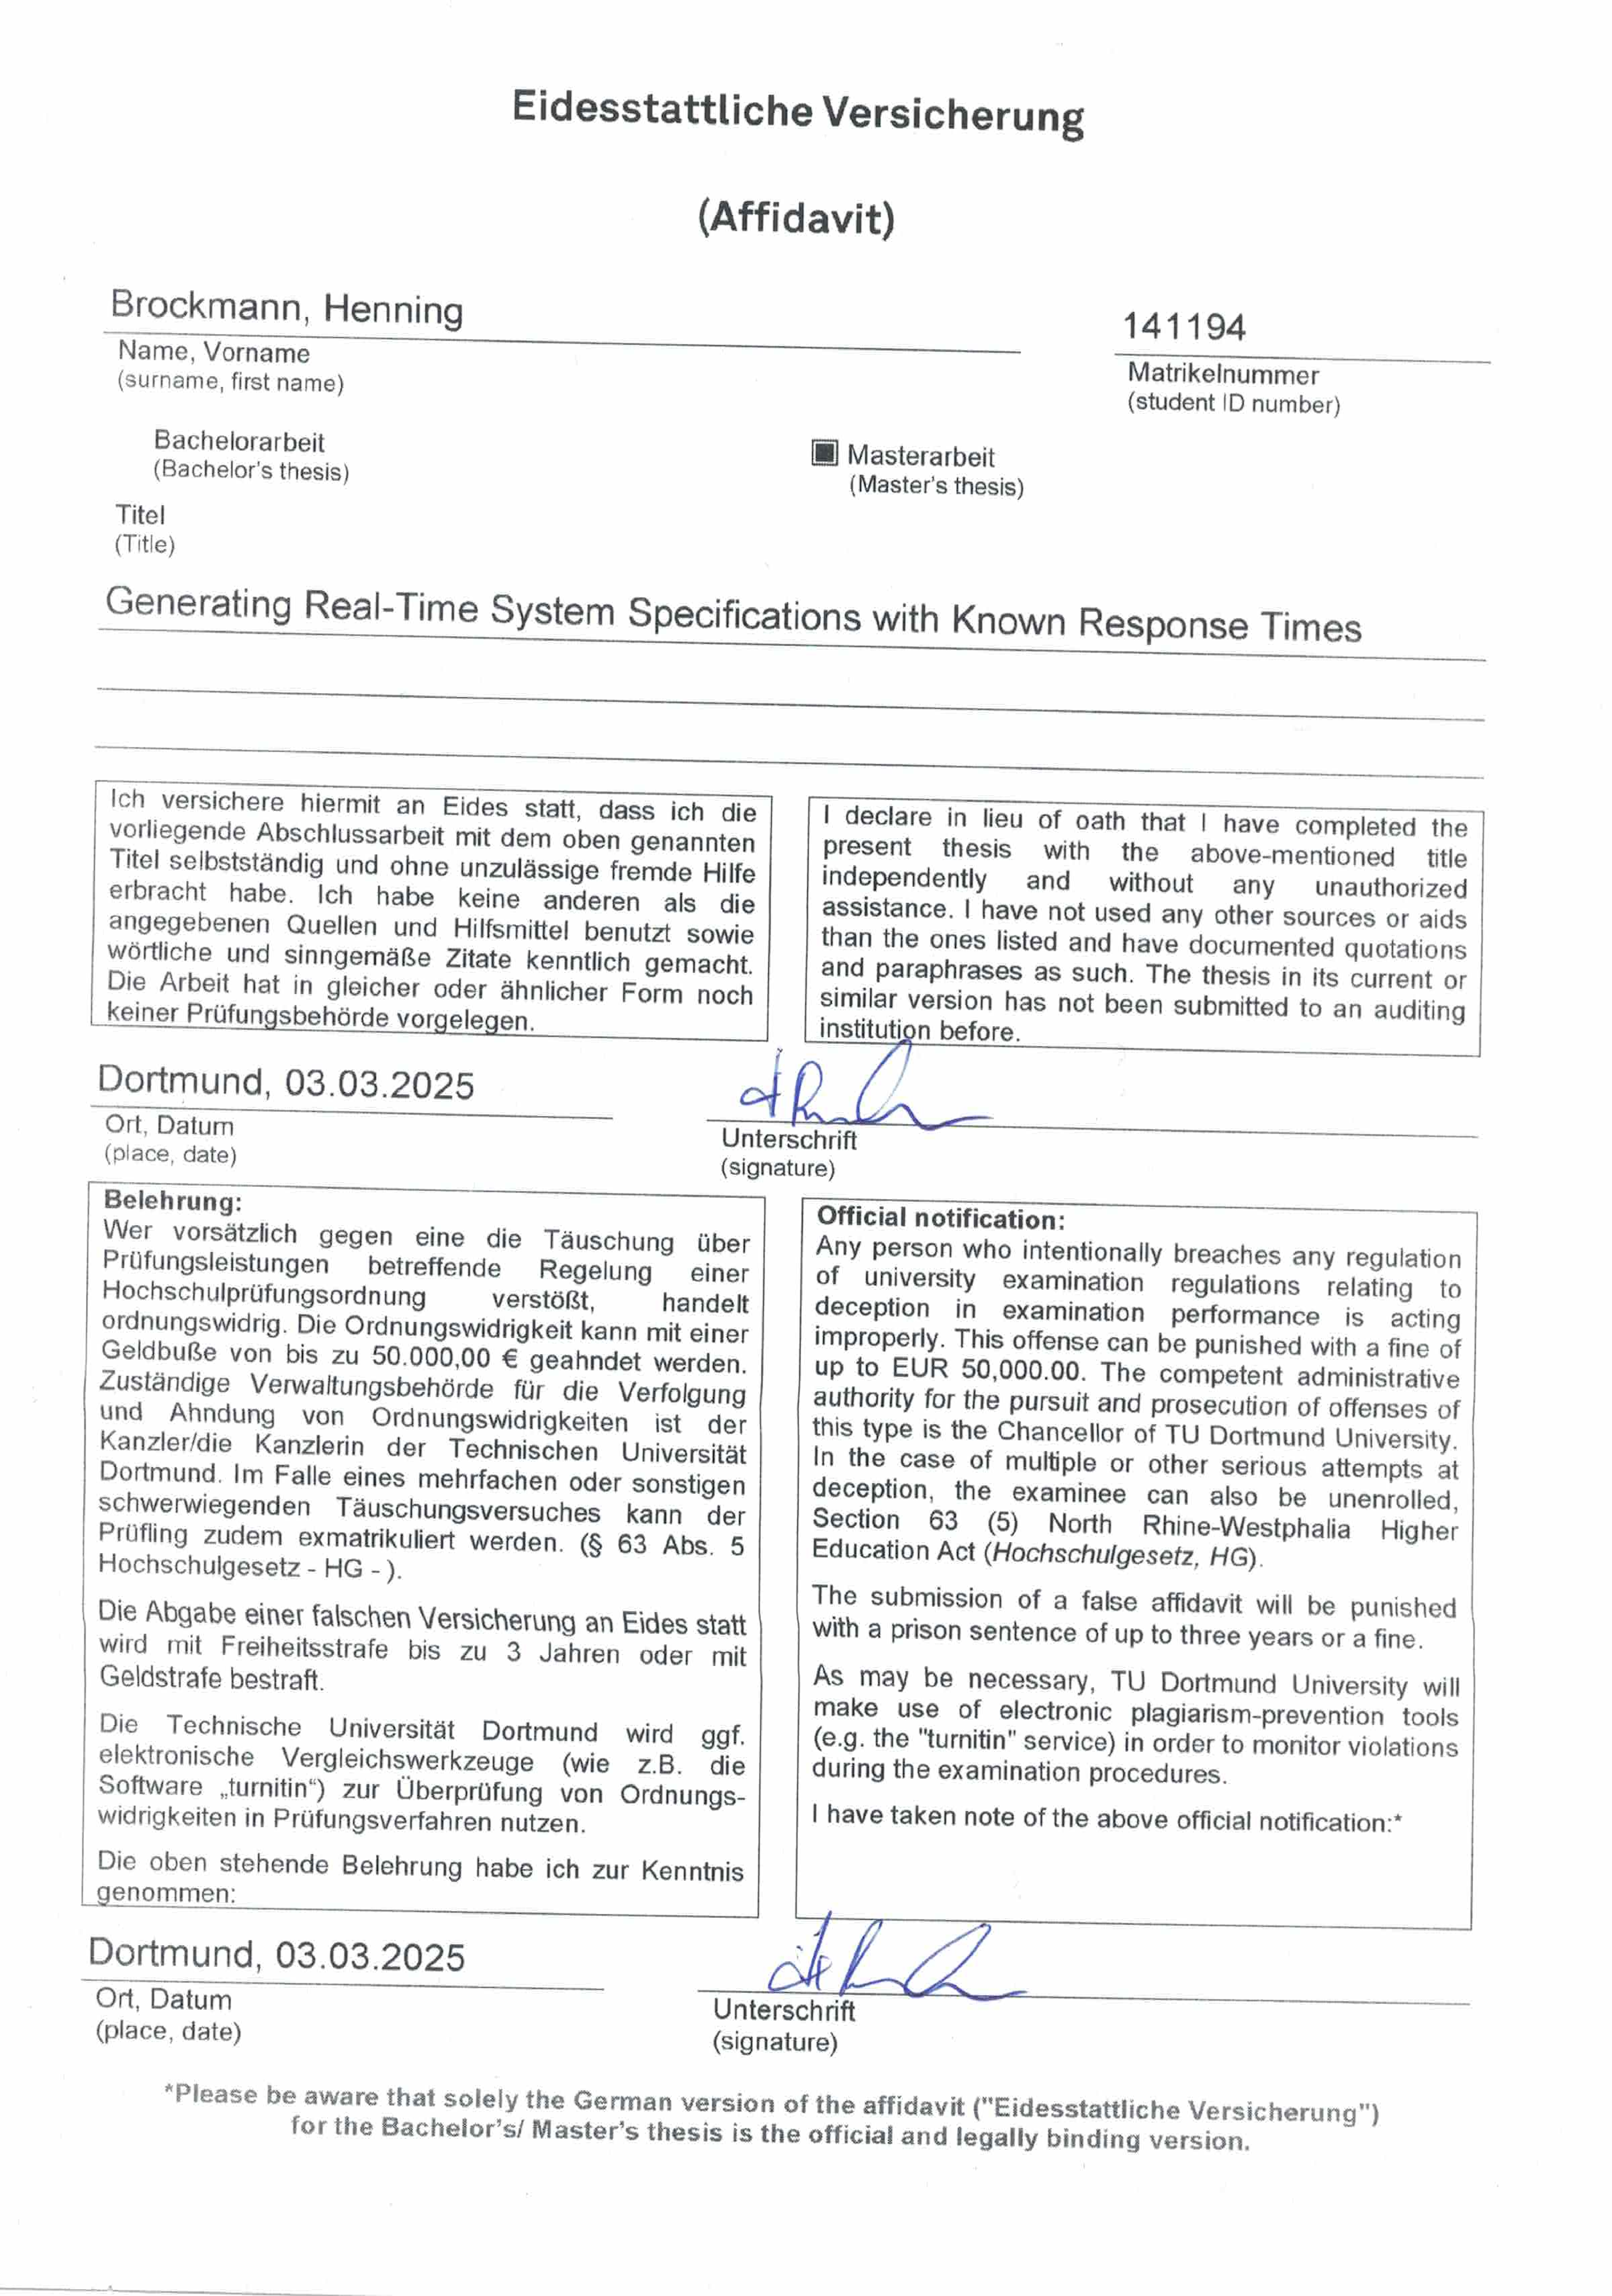
\includepdf{content/Eidesstattliche_Unterschrieben.pdf}

\end{document}
